\chapter{Dati Iniziali}

In questa sezione ci si soffermerà in quella che è una preliminare analisi dei dati iniziali a disposizione. Questi dati rappresentano il materiale grezzo dal quale \textit{estrarre} --- fare del \textit{mining}, come appunto il nome dell'attività suggerisce --- delle informazioni. \\

Usando come metafora una lavorazione meccanica, avere ben chiara la natura del materiale grezzo a disposizione consente di scegliere opportunamente gli utensili adatti per il lavoro da fare. Nel nostro caso, poter vantare di una comprensione generale di ciò che si ha a disposizione, potrà consentirci di scegliere le tecniche migliori per trarre il meglio dai dati iniziali. \\

\section{Carriera degli Studenti}

Parte fondamentale dell'analisi descritta in questo lavoro è basata su questo dataset, rappresentante i dati riguardanti la produttività di tre coorti d'immatricolazione di studenti in un periodo di quattro anni. Più nel dettaglio, il dataset si compone di:

\begin{itemize}
	\item studenti immatricolati nell'anno 2010, carriera registrata fino all'A.A. 2013-2014 compreso
	\item studenti immatricolati nell'anno 2011, carriera registrata fino all'A.A. 2014-2015 compreso
	\item studenti immatricolati nell'anno 2012, carriera registrata fino all'A.A. 2015-2016 compreso
	\item studenti immatricolati nell'anno 2013, carriera registrata fino all'A.A. 2016-2017 compreso
\end{itemize}

Quindi, si ha a disposizione una finestra temporale di risultati ottenuti nei corsi così composta:

\begin{center}
	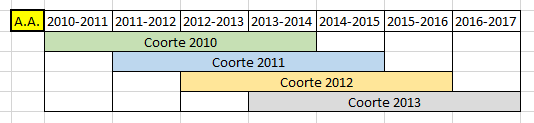
\includegraphics[scale=0.7]{../raw/stud_comp.png}
\end{center}

Questo fatto porta ovviamente ad avere una mole d'informazioni più addensata nella parte centrale della nostra finestra temporale, avendo idealmente informazioni riguardanti tutte le materie del C.d.L. solo nell'Anno Accademico 2013-2014. Questo aspetto sarà rilevante nell'interpretare i risultati di alcune analisi effettuate in seguito.

\subsection{Formato e Rappresentazione}

Il dataset è stato fornito in un unico file CSV, un formato \textit{plain text} facilmente manipolabile e interpretabile da un'ampia gamma di software. Esso si compone di una unica tabella, nella quale ogni tupla identifica uno studente, per il quale sono presenti attributi che descrivono la sua carriera universitaria nel periodo preso in esame. Oltre alle informazioni generali, quali ad esempio i risultati conseguiti nel test d'ingresso e il numero di crediti totali ottenuti nella finestra temporale esaminata, sono presenti attributi relativi alla data e al voto ottenuto in ciascun esame sostenuto. \\

Nel dettaglio, per ogni tupla rappresentante uno studente sono presenti le seguenti informazioni:

\begin{itemize}
	\item Coorte di immatricolazione: $$ \{2010, 2011, 2012, 2013\} $$
	\item Voto conseguito nel test di ingresso: $$ \{ x \in \mathbb{N} \text{ tale che } 0 \leq x \leq 25\} $$
	\item Voto ottenuto all'esame di maturità: $$ \{ x \in \mathbb{N} \text{ tale che } 60 \leq x \leq 100\} $$
	\item Tipo di scuole superiore frequentata: $$ \{LS, Lc, It, TC, IP, AL \} $$
	\item Crediti totali ottenuti: $$ \{ x \in \mathbb{N} \text{ tale che } 0 \leq x \leq 180\} $$
	\item Crediti ottenuti da esami con voto: $$ \{ x \in \mathbb{N} \text{ tale che } 0 \leq x \leq 159\} $$
	\item Voto medio ottenuto negli esami: $$ \{ x \in \mathbb{N} \text{ tale che } 18 \leq x \leq 31 \text { con 31 indicante il 30 con lode}\} $$
	\item Voto ottenuto in un dato esame: $$ \{ x \in \mathbb{N} \text{ tale che } 18 \leq x \leq 31 \text { con 31 indicante il 30 con lode}\} $$
	\item Data in cui è stato sospenuto quell'esame: $$ \text{data in formato }MM/GG/YYYY $$
\end{itemize}

\subsection{Campione del Dataset}

Di seguito si mostra un campione del dataset, al fine unico di esibirne la struttura generale. Si noti che, per ragioni evidenti di spazio, sono state omesse le colonne rappresentanti gli attributi di tutti gli esami.

\begin{center}
	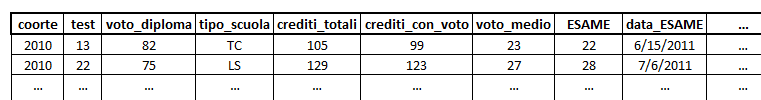
\includegraphics[scale=0.5]{../raw/stud_sample.png}
\end{center}

\section{Valutazione degli Insegnamenti}
	Lorem ispsum bla bla bla

\subsection{Formato e Rappresentazione}

\subsection{Campione del Dataset}

Analogamente a quanto fatto per l'altro dataset, si mostra di seguito un campione al solo scopo di mostrarene la struttura. Dato il fine, si è mostrato solo un ristrettissimo campione di uno dei sette dataset forniti, essendo la struttura degli altri sei totalmente identica.

% ok, now fill it!
\begin{center}
    \begin{tabular}{| l | l | l | l |}
    \hline
    Day & Min Temp & Max Temp & Summary \\ \hline
    Monday & 11C & 22C & A clear day with lots of sunshine.
    However, the strong breeze will bring down the temperatures. \\ \hline
    Tuesday & 9C & 19C & Cloudy with rain, across many northern regions. Clear spells 
    across most of Scotland and Northern Ireland, 
    but rain reaching the far northwest. \\ \hline
    Wednesday & 10C & 21C & Rain will still linger for the morning. 
    Conditions will improve by early afternoon and continue 
    throughout the evening. \\
    \hline
    \end{tabular}
\end{center}
